\section{Results}

\subsection{Baseline Model}
\begin{scriptsize}
	\vspace{-\parskip}
	\url{https://wandb.ai/mfixman-convolutional-team/work/runs/j6iippi9}
	\hfill{} Wandb tag: `\texttt{baseline}'
\end{scriptsize}

The baseline model, being extremely simple, does nearly not overfit its data.
Instead, it badly underfits the data and doesn't give the best result.

\begin{figure}[h]
	\centering
	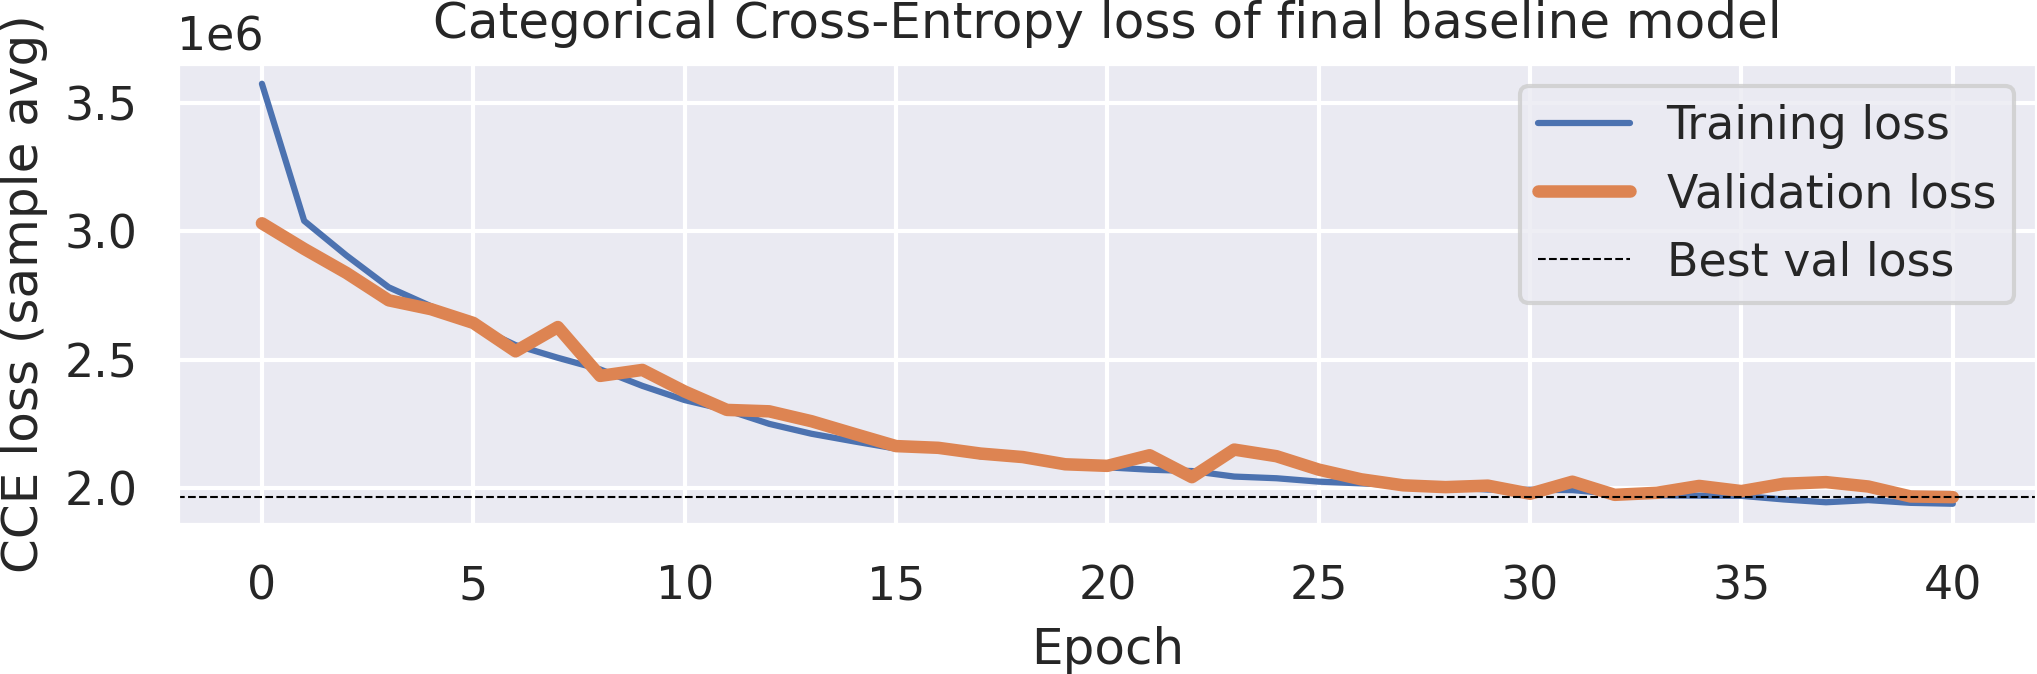
\includegraphics[width=.9\textwidth]{baseline_loss.png}
	\caption{Baseline loss by epoch}
	\label{baseline_model_loss}
\end{figure}

The results of this model are notoriously ``blocky'': while there are clusters of correct pixels where they should go, it seems the model has problems filling those clusters.
This is likely due to the small ratio between kernel size and minimum image, and the lack of skip connections which prevent it from nicely detecting the edges between different classes.

\begin{figure}[h]
	\begin{subfigure}{.5\textwidth}
		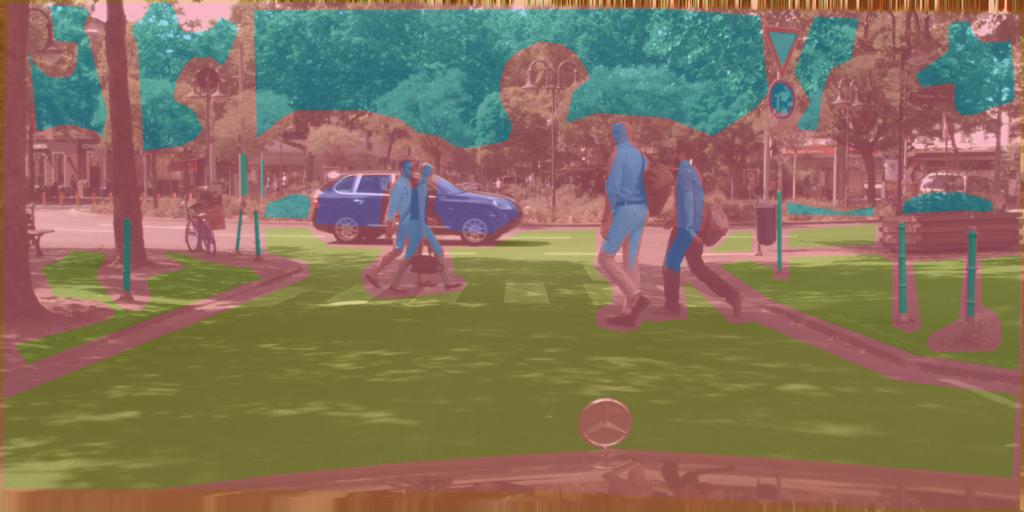
\includegraphics[width=\textwidth]{city_images/baseline_gt_pic.png}
		\caption{Ground truth}
	\end{subfigure}
	\begin{subfigure}{.5\textwidth}
		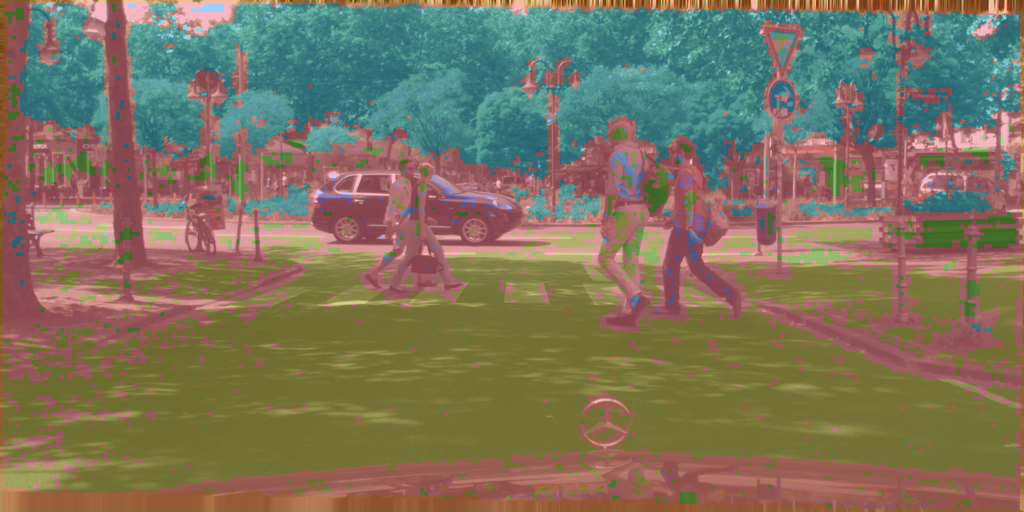
\includegraphics[width=\textwidth]{city_images/baseline_pic.png}
		\caption{Result of the baseline model.}
	\end{subfigure}
	\caption{Example result with a picture in the city of Frankfurt.}
\end{figure}

While the results are far from convincing, this works very well as a simple and light model: in this example and many others all objects (cars, people, trees, and others) are identified, regardless of how small.

It's also a fantastic starting point for a comparison.

\newpage{}

\subsection{Enhanced Model 1: UNet}
\begin{scriptsize}
	\vspace{-\parskip}
	\url{https://wandb.ai/mfixman-convolutional-team/work/runs/5ytrv216}
	\hfill{} Wandb tag: `\texttt{enhanced\_unet}' \\[-4pt]
	\url{https://wandb.ai/mfixman-convolutional-team/work/runs/qbi7duzd}\footnotemark{}
	\footnotetext{The original run got preempted and was later continued; the section shows both runs together.}
\end{scriptsize}

While the UNet model has considerably better loss than the baseline model, it overfits badly after only 15 epochs and doesn't learn much useful information afterwards.

\begin{figure}[h]
	\centering
	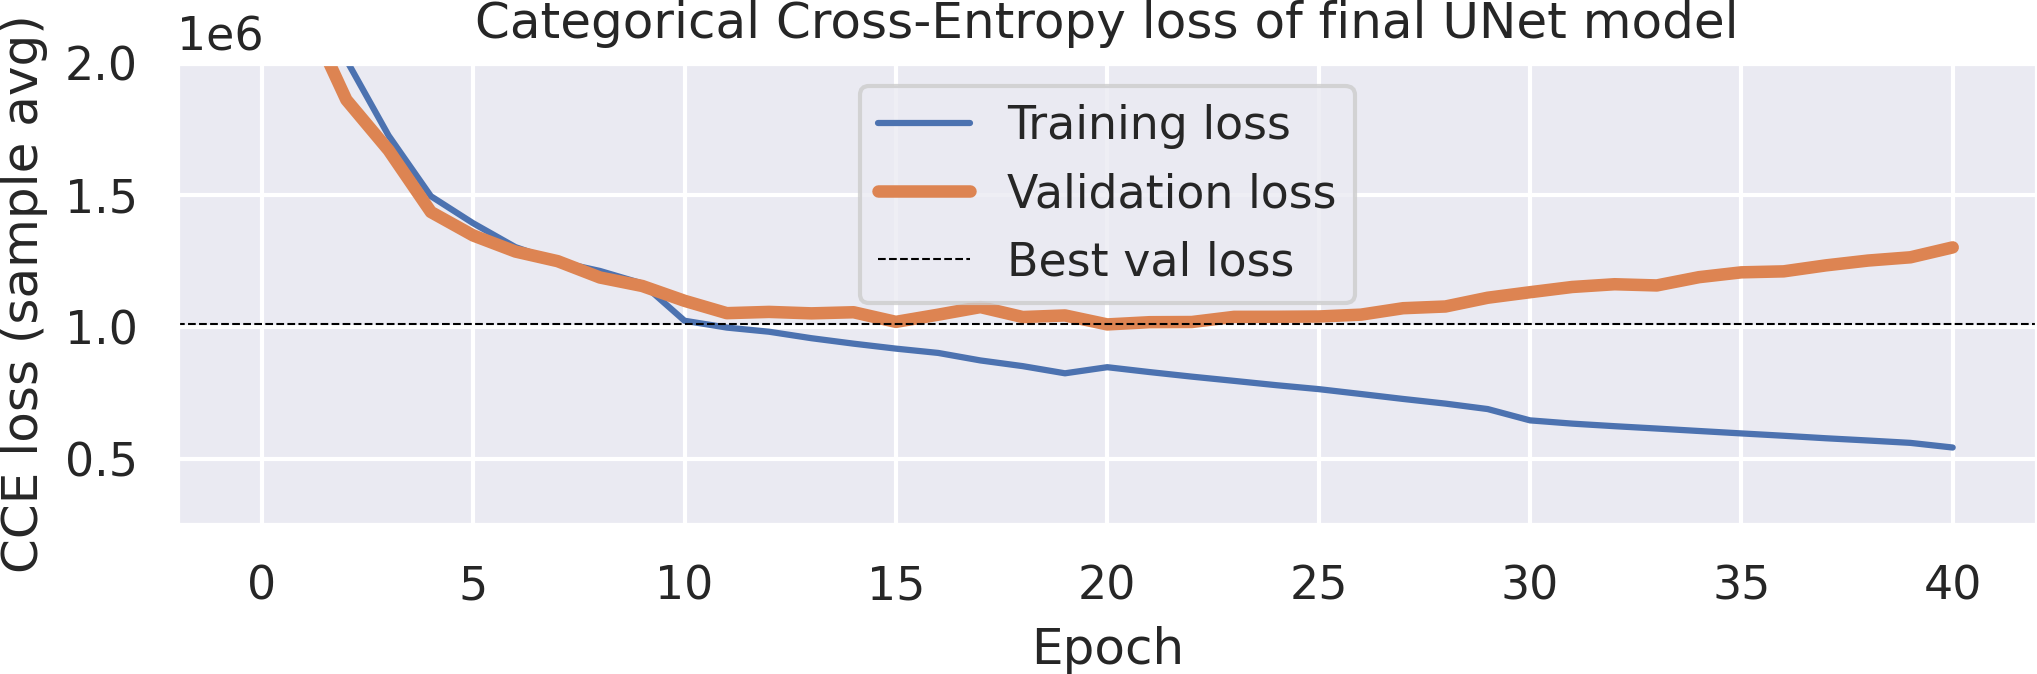
\includegraphics[width=.9\textwidth]{unet_loss.png}
	\caption{UNet model loss by epoch.}
	\label{unet_model_loss}
\end{figure}

In addition to having a good loss, it's considerably better at the task of image segmentation than the baseline model

\begin{figure}[h]
	\begin{subfigure}{.5\textwidth}
		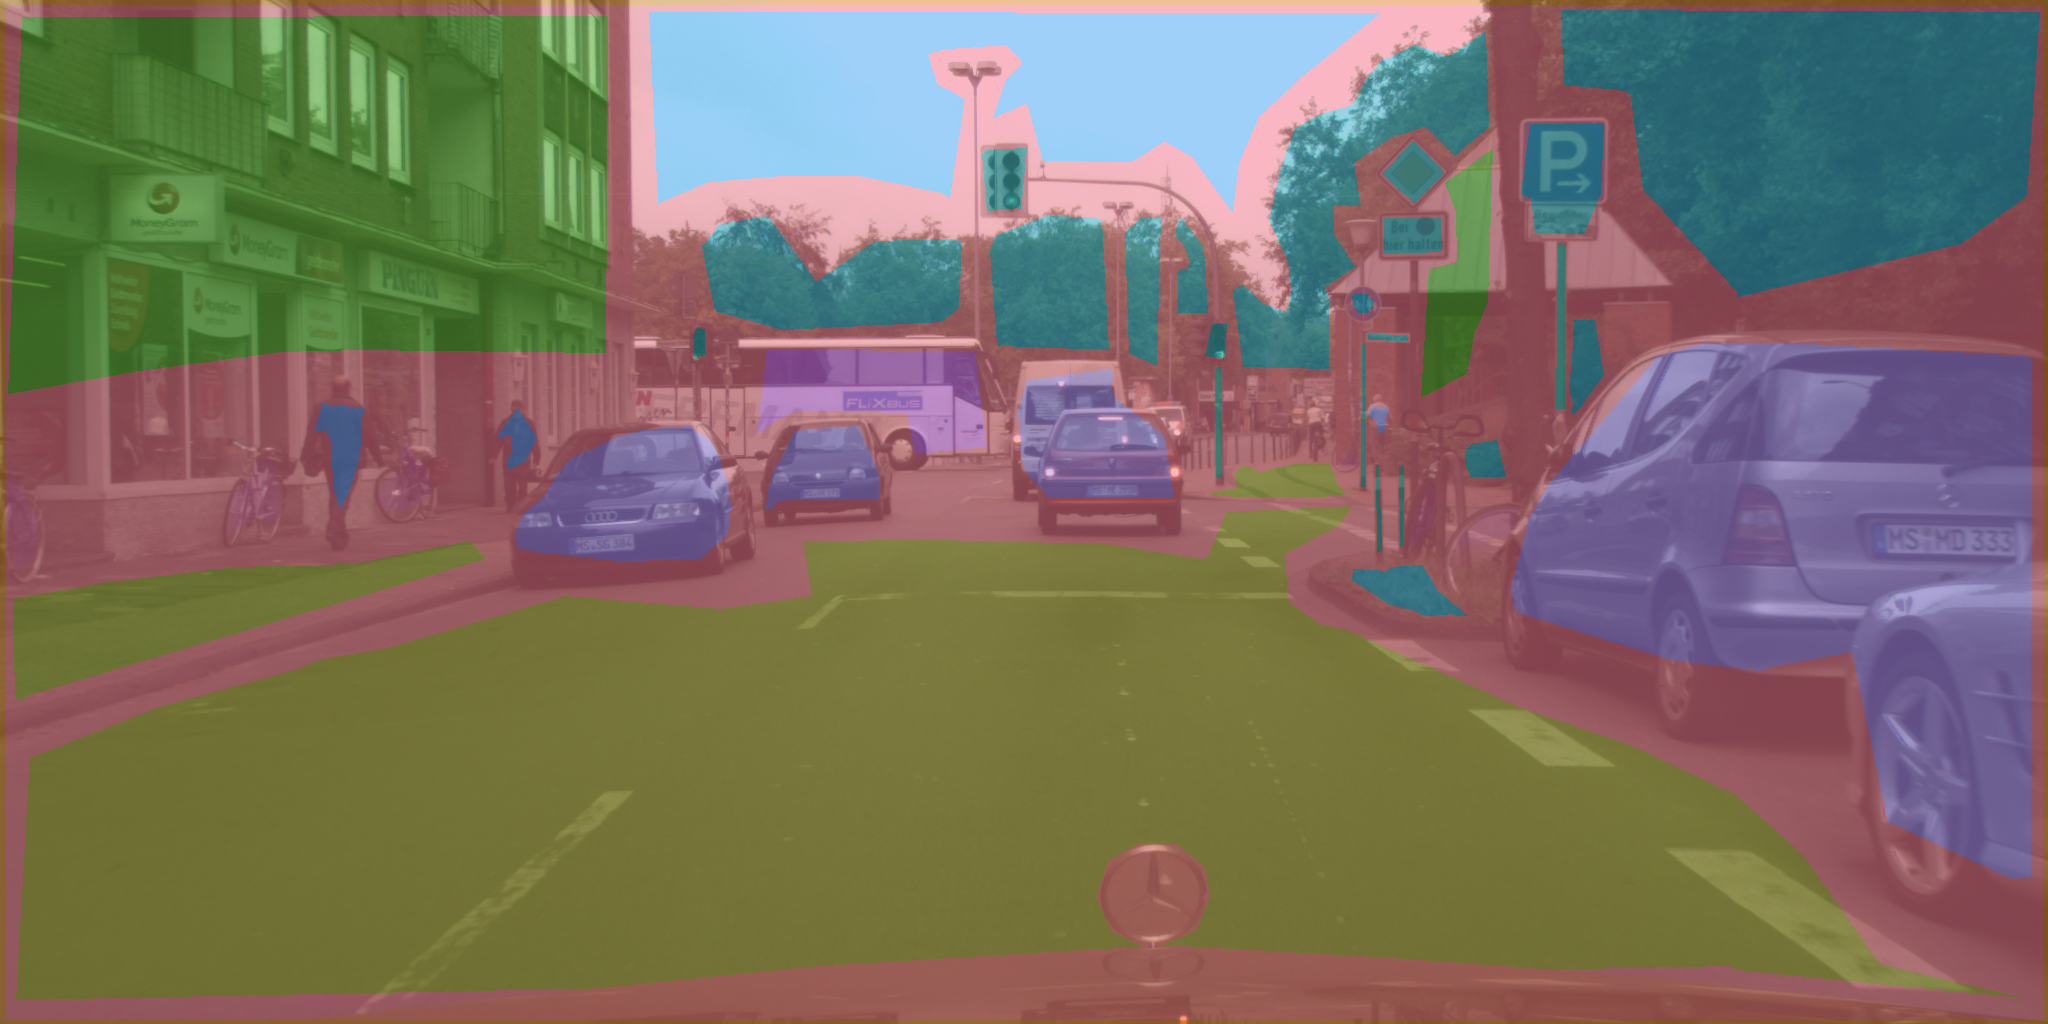
\includegraphics[width=\textwidth]{city_images/unet_gt_pic.png}
		\caption{Ground truth}
	\end{subfigure}
	\begin{subfigure}{.5\textwidth}
		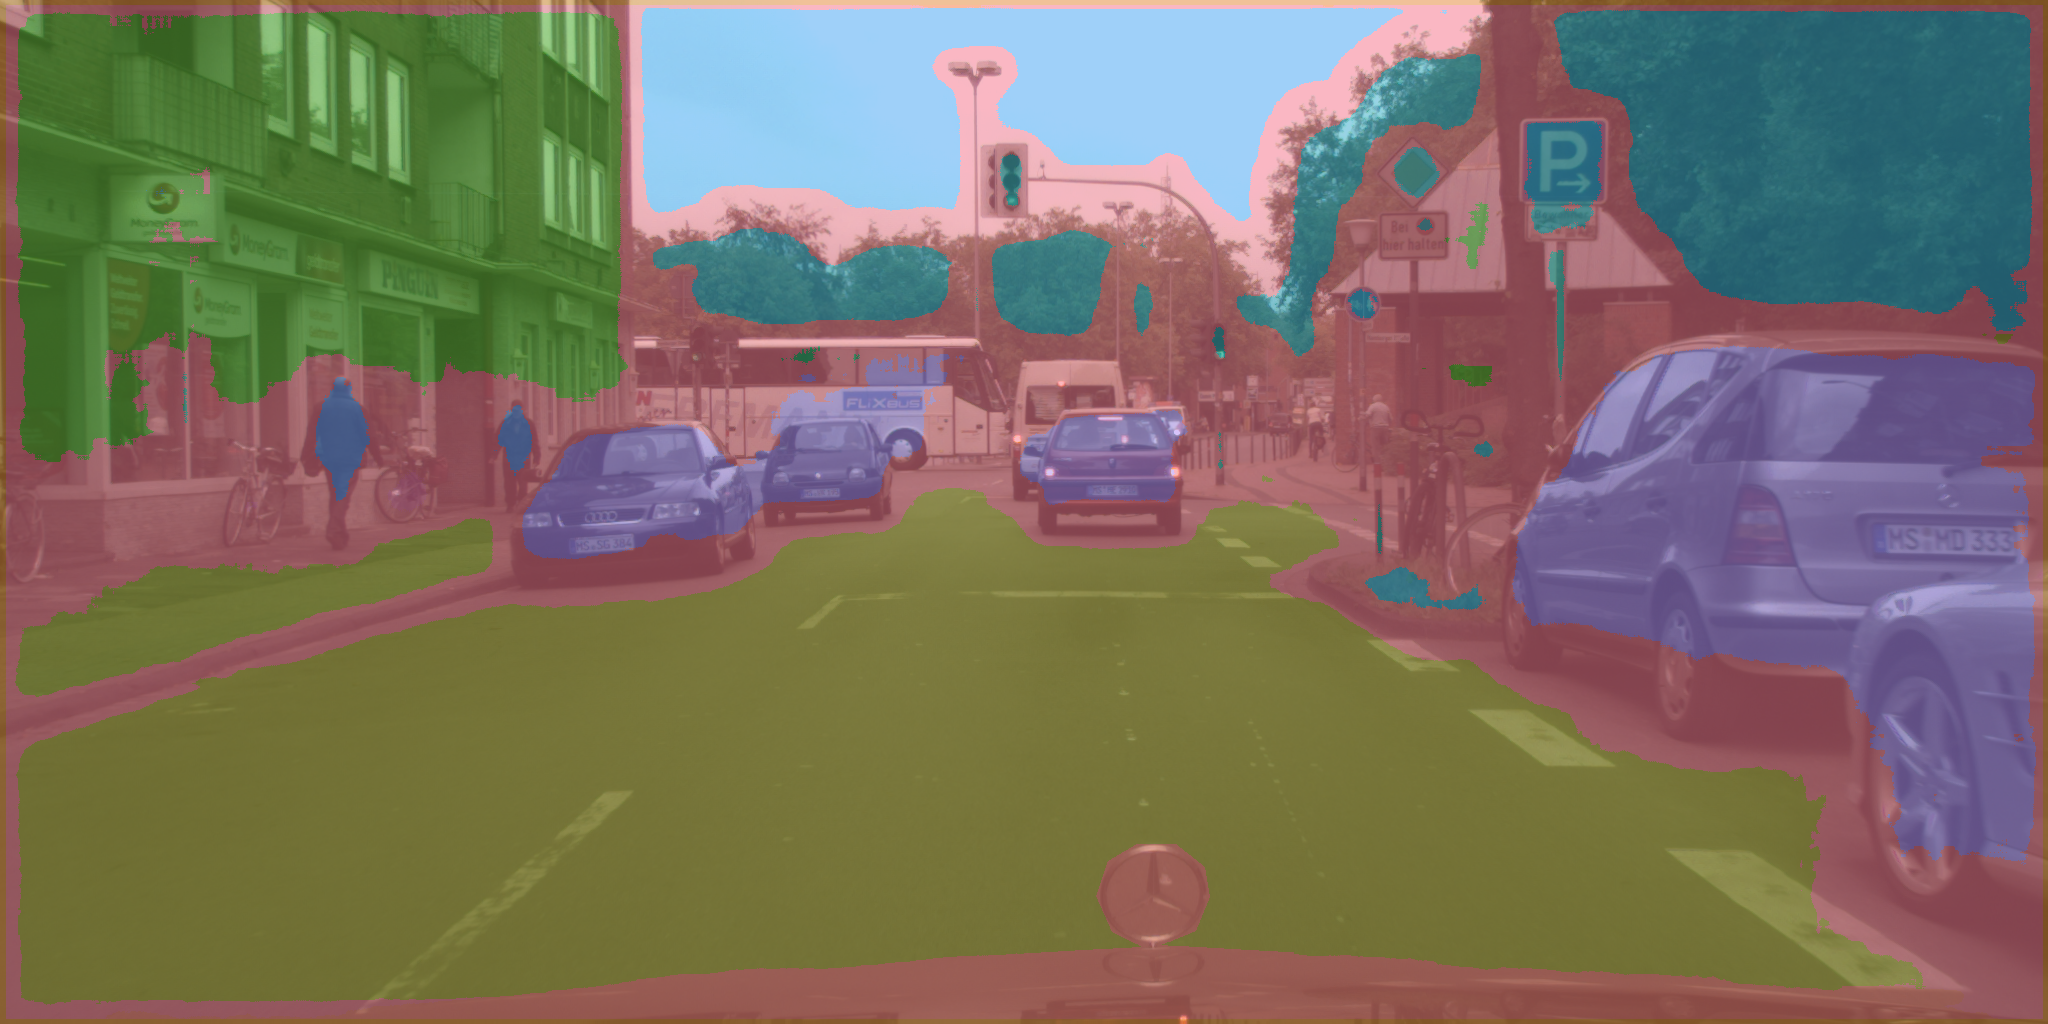
\includegraphics[width=\textwidth]{city_images/unet_pic.png}
		\caption{Result of the enhanced UNet model.}
	\end{subfigure}
	\caption{Example result with a picture in the city of Munster.}
\end{figure}

Here we can observe that the blockiness from the previous model is gone, and the filled parts are properly filled.
This is a result of how deep the encoder and decoder is, which allows it to generalise better over large patches, and of the skip connections passing data with different resolution from different parts of the encoder.

Many of the ``mistakes'' done by this model are actually caused by the arbitrariness of the coarse dataset of CityScapes.
As explained in the Reflections, this is one of the reasons why it might have been a better idea to work in the fine dataset instead.

\newpage{}

\subsection{Enhanced Model 2: Swin2}
\begin{scriptsize}
	\vspace{-\parskip}
	\url{https://wandb.ai/mfixman-convolutional-team/work/runs/sty5iun8}
	\hfill{} Wandb tag: `\texttt{enhanced\_swin2}'
\end{scriptsize}

While the Swin2 model has the lowest validation loss of all three models, this isn't comparable since this loss ignores pixels that are marked as ``background'' in the ground truth.

The dropout and pre-trained weights seem to slow its overfitting, and despite considerable overfitting of the training set after 20 epochs the model still learns relevant information.
The validation loss is at its minimum after 28 epochs.

\begin{figure}[h]
	\centering
	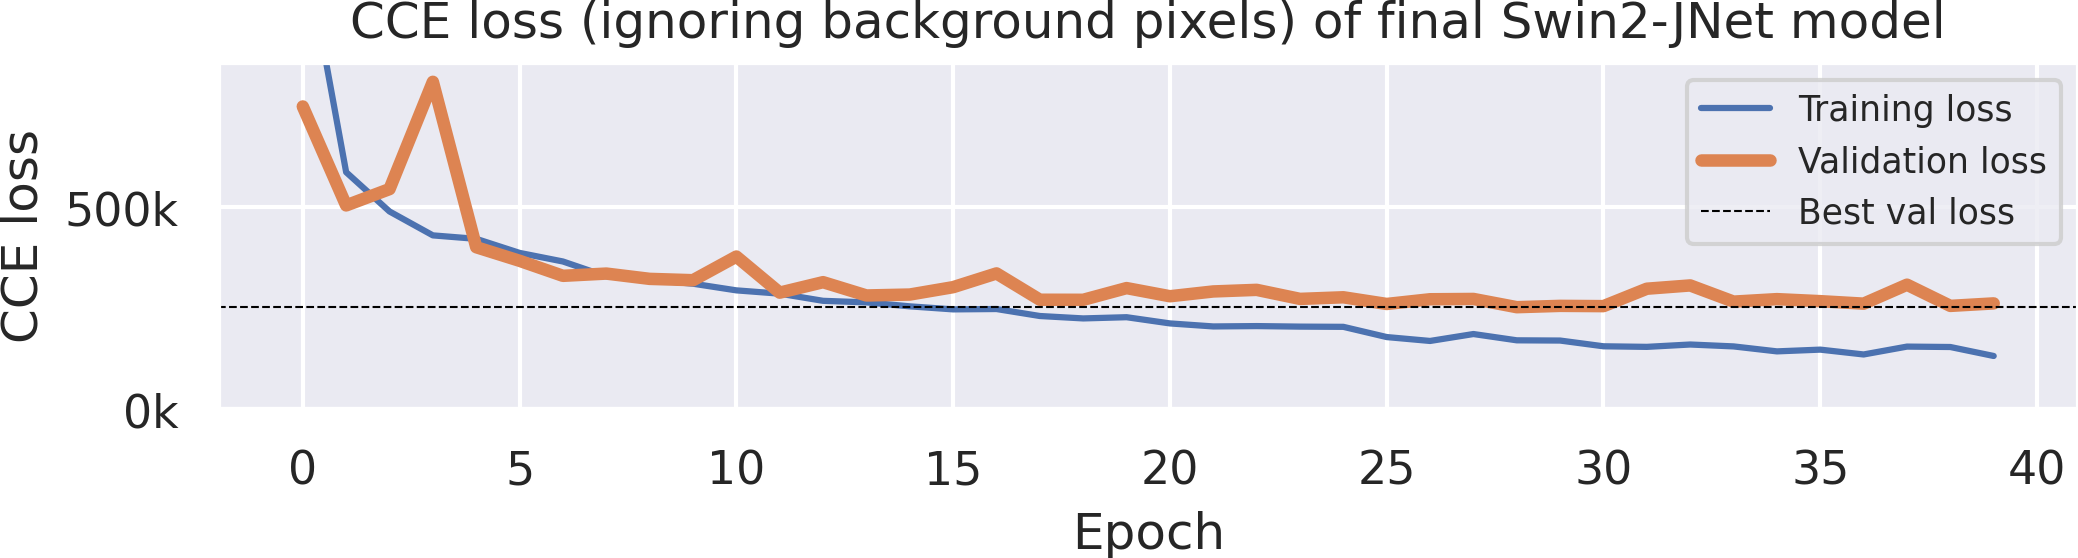
\includegraphics[width=.9\textwidth]{swin2_loss.png}
	\caption{Swin2-JNet loss by epoch.}
	\label{swin2_model_loss}
\end{figure}

The pre-trained weights in the transformer encoder seem to capture a lot of relevant picture information; this is layer re-trained in the context is CityScapes by the decoder.
This shows the promise of transfer learning: by only requiring to learn small but relevant details of the image, we can achieve a good loss in just a bit of training.

\begin{figure}[h]
	\begin{subfigure}{.5\textwidth}
		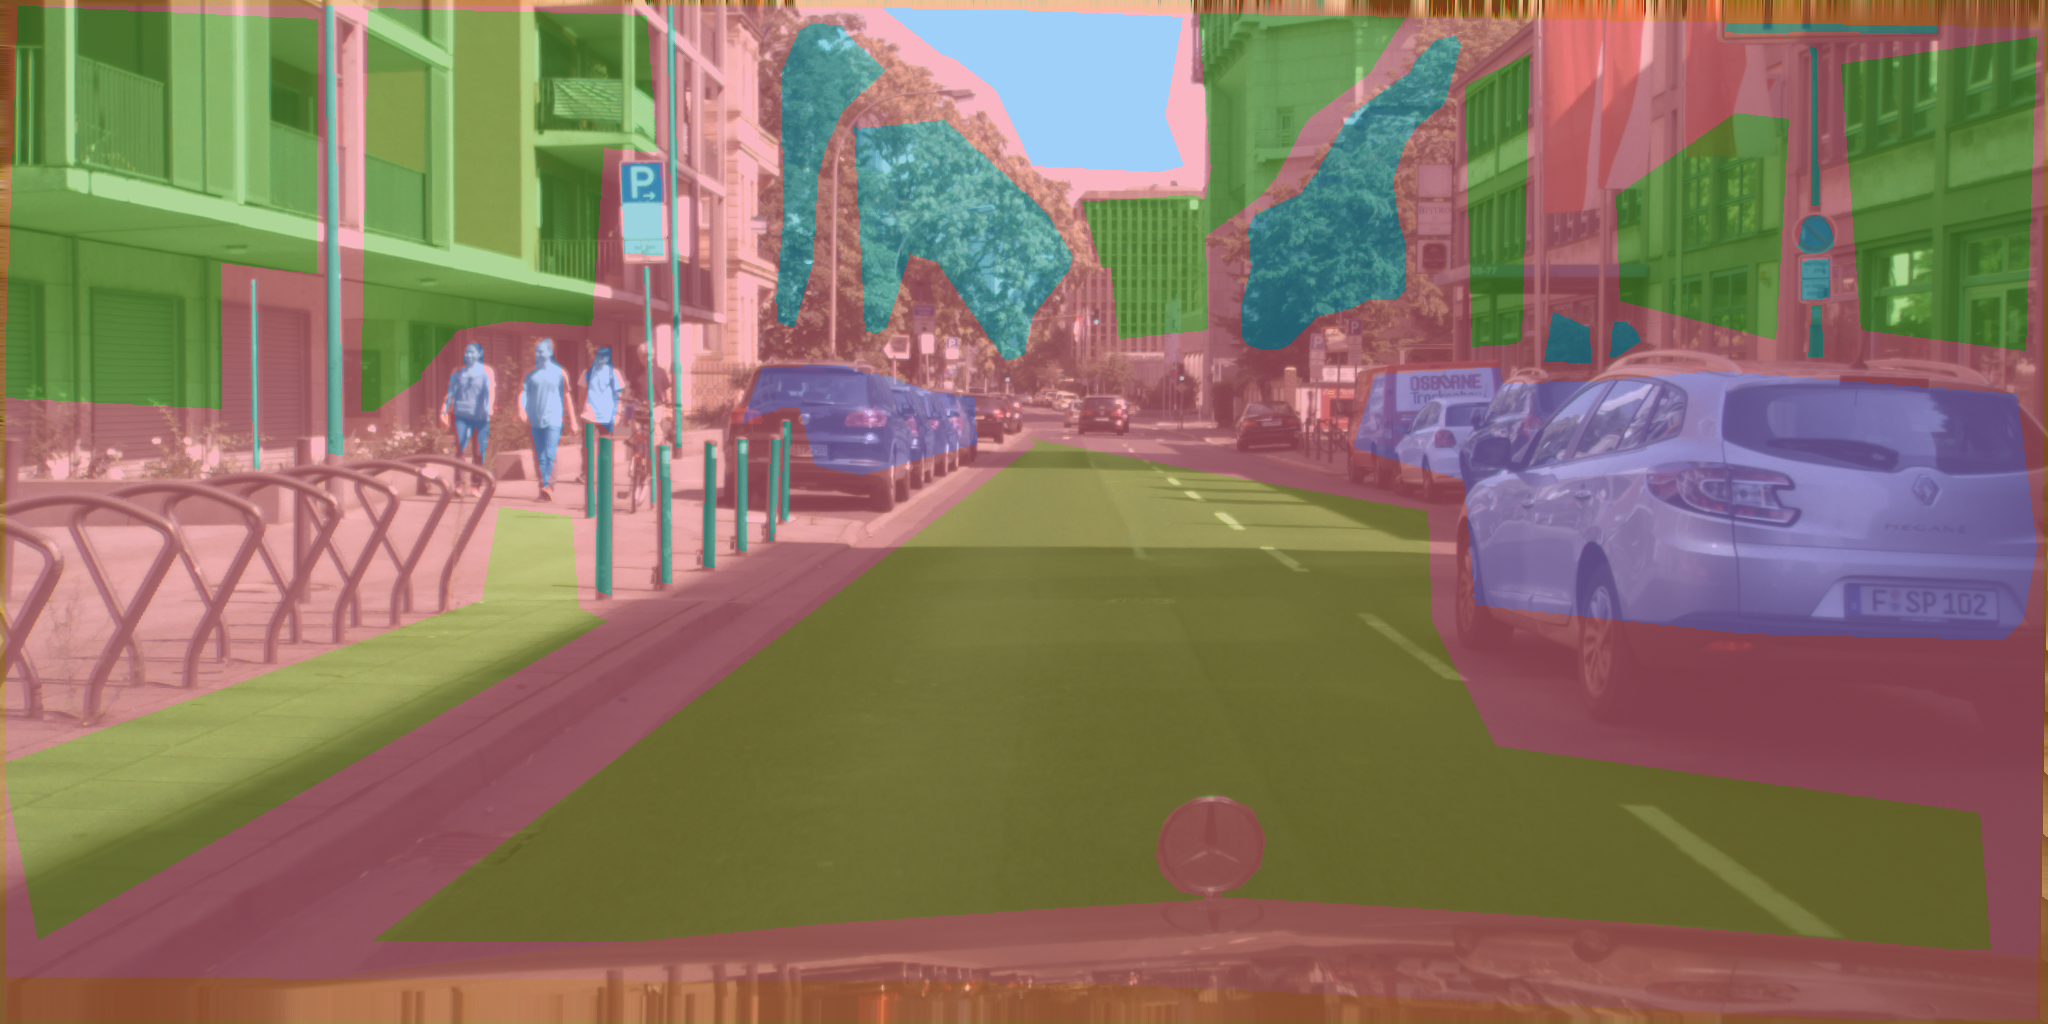
\includegraphics[width=\textwidth]{city_images/swin2_no_background_gt_pic.png}
		\caption{Ground truth}
		\label{swin2_gt_image}
	\end{subfigure}
	\begin{subfigure}{.5\textwidth}
		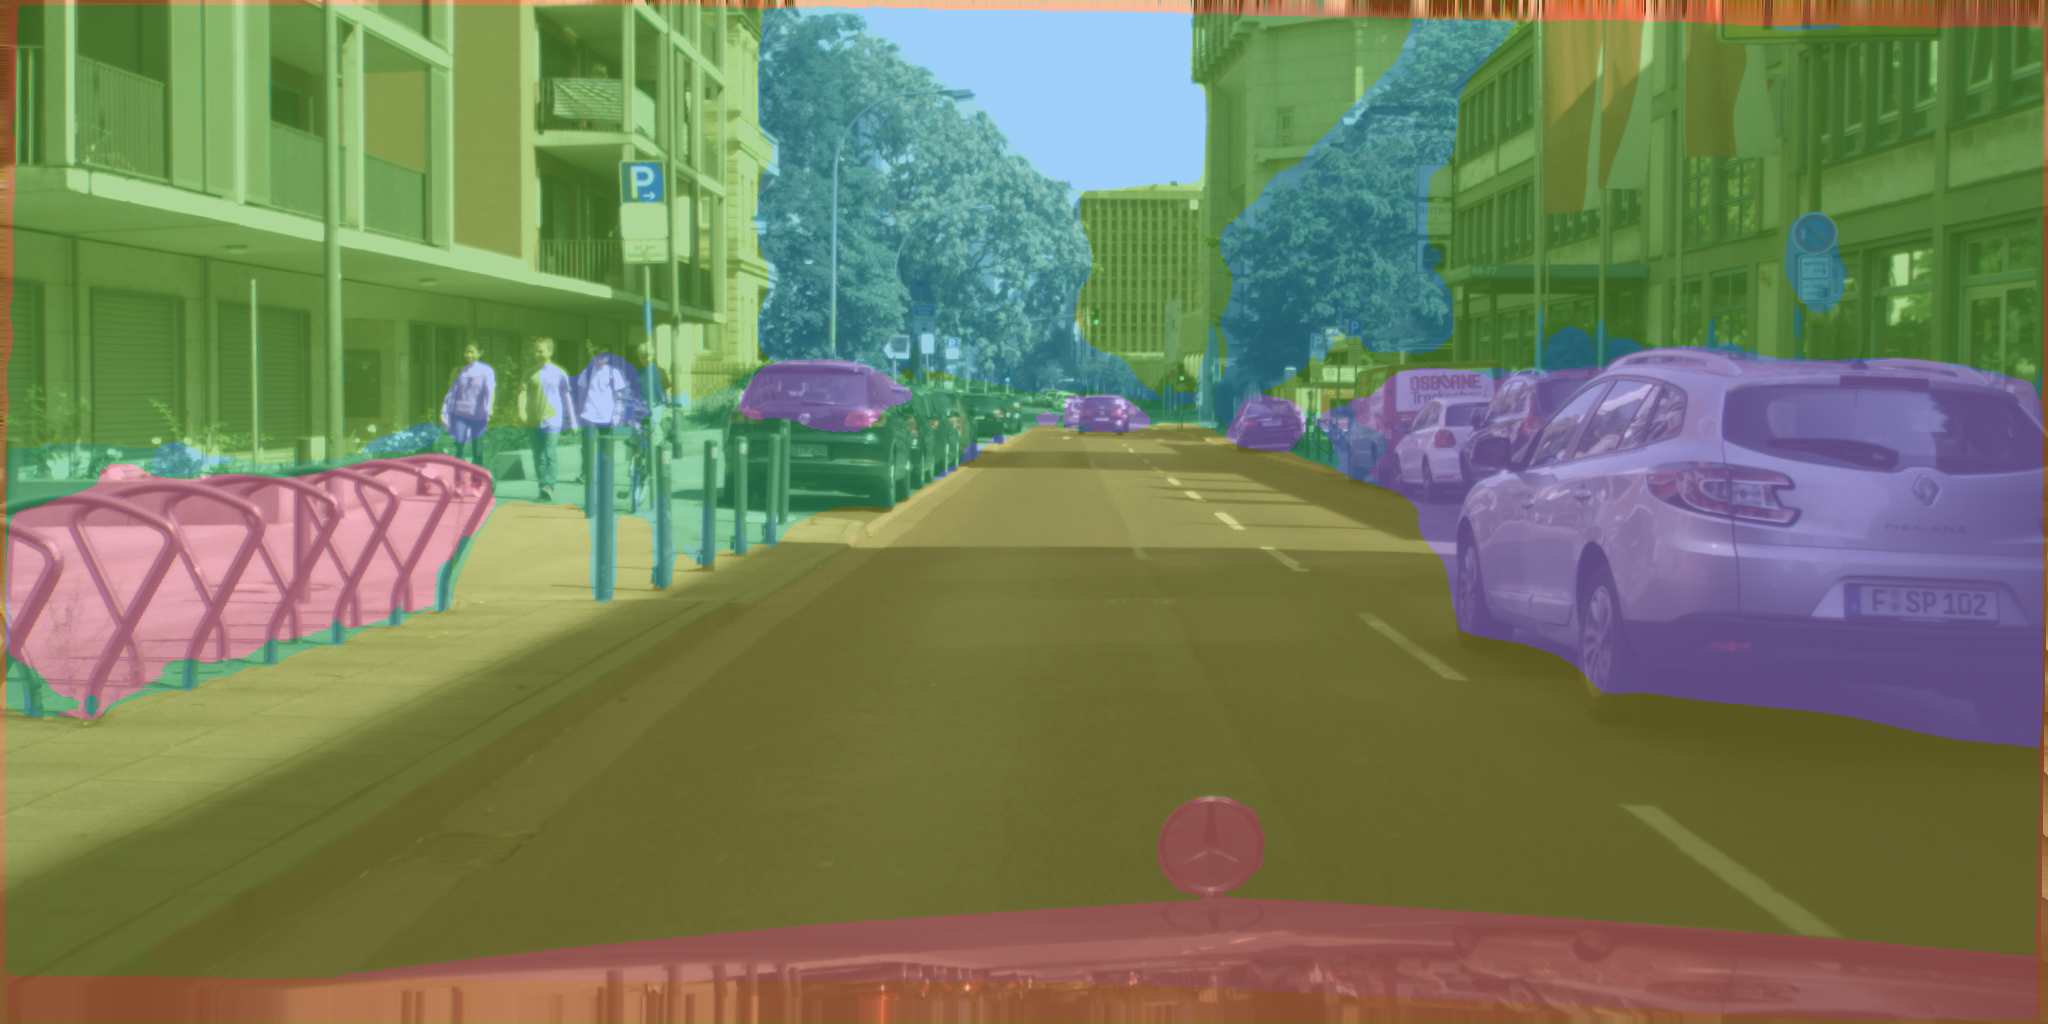
\includegraphics[width=\textwidth]{city_images/swin2_no_background_pic.png}
		\caption{Result of the enhanced Swin2-JNet model.}
		\label{swin2_result_image}
	\end{subfigure}
	\caption{Example result with a picture in the city of Munster. \textbf{\textcolor{BrickRed}{Red}} pixels are background pixels in ground truth, and unknown pixels in result.}
\end{figure}

Models trained to ignore background pixels can make good guesses to what those background pixels are.
While previous models were small enough to ``hallucinate'' these results and produce false positives, Swin2-JNet is considerably better at inferring these classes.

Many pixels in \cref{swin2_result_image} contain correct information that was masked in \cref{swin2_gt_image}.

\newpage{}

\subsection{Comparisons}
\label{comparison_section}

\begin{figure}[h]
	\centering
	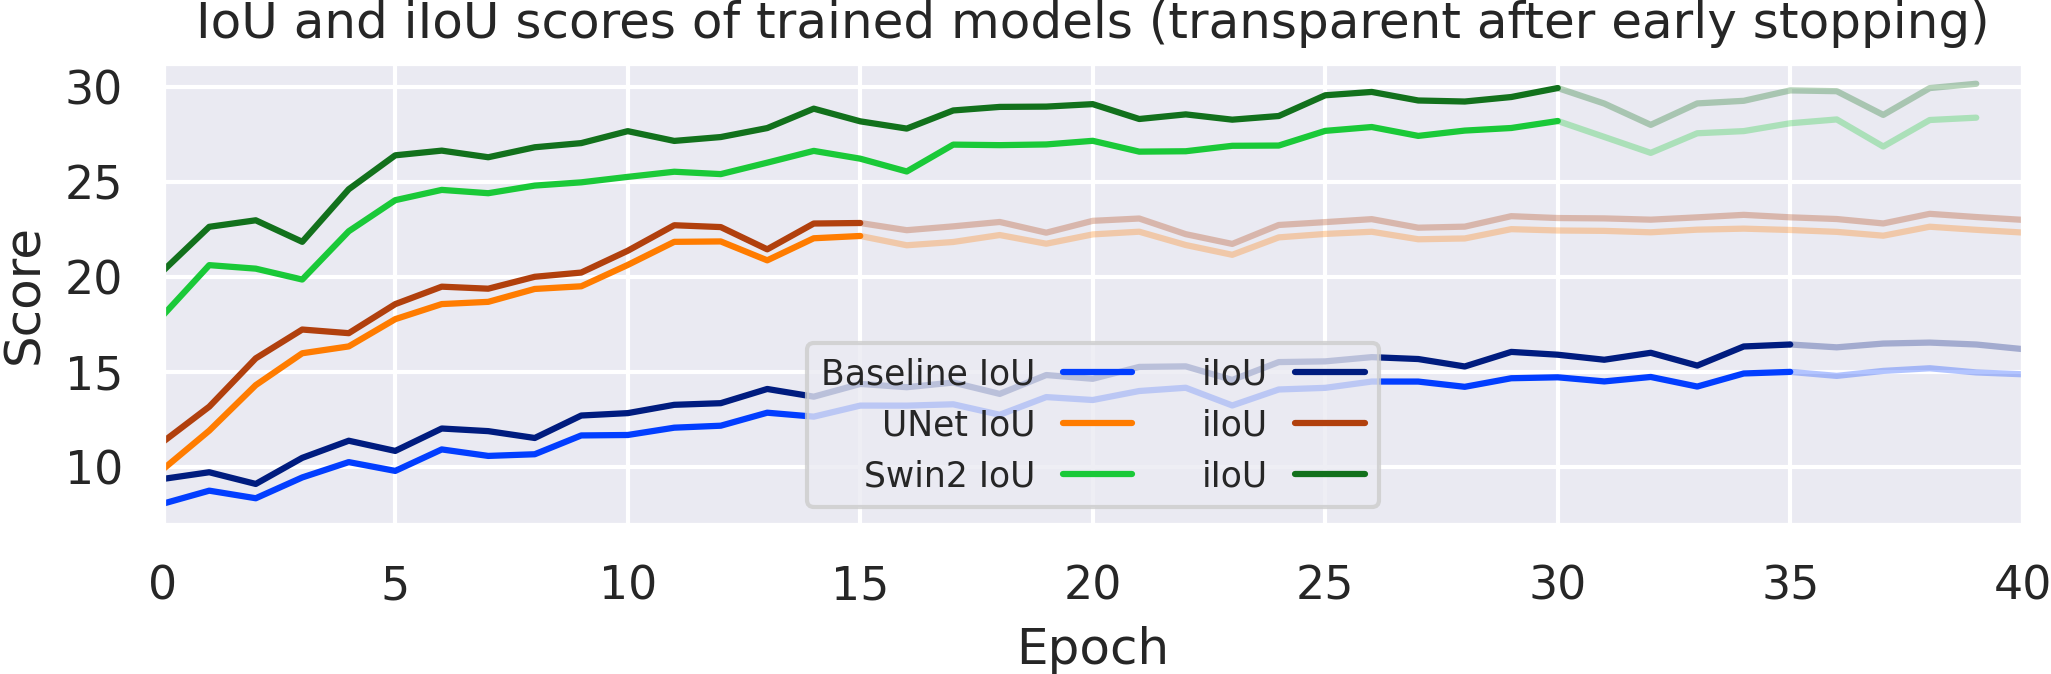
\includegraphics[width=.8\textwidth]{iou_scores.png}
	\caption{IoU and \iiouc{} scores of the three classifiers}
	\label{comparisons}
\end{figure}

We previously discussed the necessity to use common metrics about the images other than the categorical cross-entropy used for the loss.
\Cref{comparisons} shows the intersection-over-union and class intersection-over-union scores of each classifier.

% Surprisingly, in none of the classifiers there is much of a difference between these scores.
% This might happen since all our models are deep and can detect both large and small features pretty well.
% Additionally, the coarse dataset does not include much data about smaller objects.

We can clearly see that, in the first two cases, the IoU scores follow closely their categorical cross-entropy loss, which means that this loss is a good way to learn the general case.
Additionally, the \iiouc{} score trails closely to the IoU score despite none of the model being trained with weights; this is both due to the abilities of the classifiers to find small details, and also to the coarseness of the coarse dataset.

What's surprising is that the IoU score of the Swin2 model is considerably higher than the rest, despite ``wasting'' processing power in learning data about background pixels.
This is likely due to its ability to generalise: despite not having ground truth, the neighborhood values of these background pixels provide useful information for the model.

\subsection{So which model is better?}
\label{which_one_wins}

\begin{table}[h]
	\centering
	\footnotesize
	\begin{tabular}{>{\bfseries}r | r r r r}
		\toprule
		Model & CCE Loss & IoU Score & iIoU Score & Dice Loss \\
		\midrule
		Baseline & \num{1844272} & 15.64 & 16.91 & 0.97 \\
		UNet & \num{1018490} & 22.16 & 22.84 & 0.97 \\
		Swin2-JNet & \num{869488} & 28.17 & 29.93 & 0.97 \\
		\bottomrule
	\end{tabular}
	\caption{Comparison of losses between three models}
	\label{result_scores}
\end{table}

% In \cref{loss_function_section} we considered using the dice loss as either a loss or a score function to compare these results.
Initial experiments were inconclusive, and the results in \cref{result_scores} confirm this: despite having identical dice loss, the three models are wildly different.

The validation scores in \label{result_scores} show the Swin2 model to be the clear winner in CityScapes dataset.
However, does it generalise well?

We introduce ``HackneyScapes'', a series pictures taken by us in the London borough of Hackney to use as a testing set.
As we have no ground truth, these have to be tested by subjective measures in \hyperref[hackneyscapes]{Appendix A}.

Our subjective eyes confirm our metrics: \textbf{the Swin2-JNet model is clearly the winner!}
